\chapter{Módulo de Contabilidad}

%\section{Conceptos generales de Contabilidad}

\section{Clientes}

En la sección de \textbf{clientes} de este módulo se encuentran las distintas opciones en relación a los datos contables sobre los mismos. Desde las facturas a recibos e incluso los mismos datos de clientes y sus fichas.

\subsection{Facturas de clientes}
Esta opción da acceso al área de la aplicación donde se almacenan las facturas realizadas a los clientes (las facturas de ventas). Desde aquí pueden crearse nuevas facturas y ver de un vistazo las ya existentes y algunos de sus datos más importantes.

A pesar de que desde aquí pueden crearse nuevas facturas, hay que recordar que algunas son generadas automáticamente a través de los pedidos de ventas. Los encargados del control y aprobación de facturas deberán estar atentos a las nuevas facturas generadas automáticamente como borrador, que aparecen en azul en el listado, verificando que los datos introducidos son correctos para validar y generar la factura a enviar al cliente.

\begin{figure}[H]
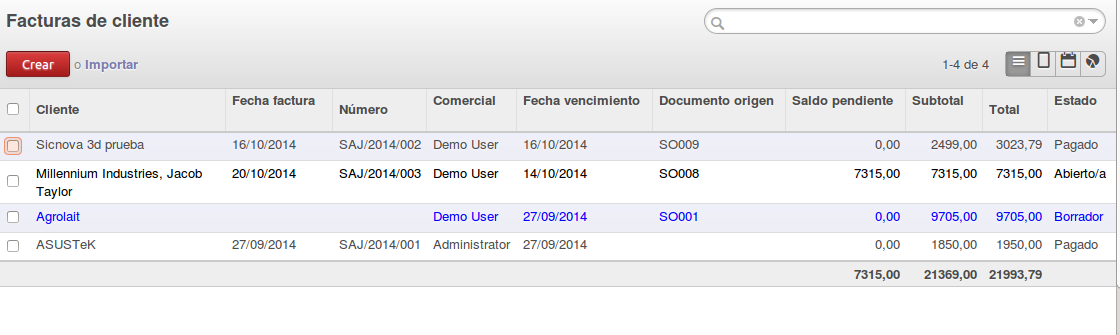
\includegraphics[width=\textwidth]{contabilidad/img/con_lisfact2.png}
\caption{Listado de facturas}
\label{con:lisfact}
\end{figure}


En el listado de facturas (figura \ref{con:lisfact} ) se ven los datos principales de las mismas. El \textbf{Cliente} al que hace referencia la factura, la \textbf{Fecha factura} de cuando fue creada, el \textbf{Número}, que no es más que la numeración de la factura, la cual es además personalizable. 

El \textbf{Comercial} hacereferencia a quién ha gerenardo la factura. Si la factura se crea a mano, este campo será el del usuario
que la ha creado. Si la factura ha sido generada automáticamente a través de una orden de venta, por ejemplo, este campo se rellenará con el nombre del comercial que ha generado dicha orden de venta. De igual manera, el campo \textbf{Documento origen} hará referencia a ese documento (orden de venta, por ejemplo) que ha generado automáticamente la factura.

La \textbf{Fecha de vencimiento} indica, en el caso de utilizar \emph{plazos de pago}. Esta fecha de vencimiento se genera automáticamente de acuerdo a estos plazos. Cuando se utilizan plazos de pagos, se generarán automáticamente los asientos contables en distintas fechas (para por  ejemplo pagos de 50\% en un plazo y el resto en otra fecha, adaptando este campo a estas fechas de asientos. También pueden no utilizarse plazo de pago y forzar una fecha de vencimiento concreta. O no utilizar ni fecha de vencimiento ni plazo de pago, indicando de esta manera que el pago es directo.

El \textbf{Saldo pendiente} indica el dinero pendiente de pago de esa factura. El campo \textbf{Subtotal} muestra el total a facturar \textbf{sin} contar con los impuestos, mientras que en el campo \textbf{Total} si muestra la facturación total incluyendo los impuestos.

El \textbf{Estado} de la factura, cuyos posibles estados son los siguientes:

\begin{itemize}
  \item \textbf{Borrador} -- Estado por defecto para las nuevas facturas. En este punto, las facturas \emph{son todavía editables en todos sus
                             campos}
  \item \textbf{Pro-forma} -- Si el sistema tiene activada la capacidad de generar facturas pro-forma, este estado se encontrará disponible. En
                             este punto, la factura no tiene aún una numeración asignada.
  \item \textbf{Abierto/a} -- En este estado, la factura está confirmada, y se mantiene en este estado hasta que se realiza el pago completo
                             de la misma. Al llegar a este estado, las facturas \emph{no permite editar todos sus campos}, no se pueden cambiar
                             las líneas de factura y otros elementos. Si fuera necesario cambiarlos, habría que \emph{Cancelar} la factura, editarla
                             y volver a aprobarla.
  \item \textbf{Pagada} -- Estado al que se llega automáticamente al introducir el pago (o los pagos) de la factura. Los asientos de estos pagos pueden
                           o no estar conciliados, esto no es relevante para el cambio de estado.
  \item \textbf{Cancelada} -- Estado al cancelar la factura. Las facturas canceladas que ya han sido numeradas (que han pasado por el estado de
                           abierto) \textbf{no pueden ser borradas}, hay que pasarlas a borrador, editarlas con la nueva información
\end{itemize}


\subsubsection{Factura individual}

La figura \ref{con:facindividual} muestra la visión individual de una factura con su pestaña \emph{Líneas de factura} seleccionada. Además de esta pestaña hay otras dos denominadas \emph{Otra información} y \emph{Pagos}

\figura{contabilidad/img/con_facindividual.png}
{Vista individual de edición de una factura}
{con:facindividual}

Al seleccionar en el campo de \textbf{Cliente} uno ya existente, la factura se rellenará automáticamente con los datos de dirección y facturación introducidos en la ficha del cliente, no siendo necesario volver a repetirlos en la factura.

Se debe seleccionar la \textbf{Posición fiscal} si procede y añadirla fecha de la factura si no está completada (si no es una factura creada
automáticamente)

El campo de \textbf{Cuenta} se rellena automáticamente según el cliente, indica en que cuenta se crearán los asientos contables de esta factura  (no incluyendo los impuestos, por supuesto)

En la imágen se puede apreciar también la \textbf{pestaña Líneas de factura}. En esta pestaña se introducen las líneas de facturación, es decir, los productos incluidos en esta factura. Pulsando sobre el texto \emph{Añadir un elemento} se creará una nueva línea en la que se podrá elegir el producto a incluir a través de la columna \emph{Producto}. Al seleccionar el producto se rellenarán automáticamente el resto de campos. Estos se rellenarán con los datos introducidos previamente en el producto, pero pueden ser editados in situ en cada línea, por ejemplo. \textbf{A cada cambio que pueda afectar al precio} se debe, tras el susodicho cambio, pulsar en \emph{(actualizar)}, situado justo encima del calculo total de la cantidad de la factura.

Como \textbf{Plazos de pago} existen algunos por defecto, siendo totalmente configurable según las necesidades de la venta.

De igual forma, el campo de \textbf{Información adicional} se puede utilizar para almacenar cualquier información extra en relación a la factura.


\figura{contabilidad/img/con_pesotra.png}
{Pestaña \emph{Otra información} de una factura}
{con:pesotra}

La figura \ref{con:pesotra} muestra la \textbf{pestaña de \emph{Otra información}}. En la misma se puede observar algunos campos no relacionados de forma totalmente directa con la factura como el \textbf{Comercial} y \textbf{Equipo de ventas} responsables de la factura   el \textbf{Documento origen}-- rellenado automáticamente si la factura se genera automáticamente desde otro documento.

La \textbf{Referencia del cliente} es rellenada automáticamente en el caso de que exista dicha información en la ficha del cliente. De igual forma la \textbf{Cuenta bancaria}, campo que hace referencia al número de cuenta contra el que se pagará la factura, se extrae automáticamente de la ficha del cliente en el caso de que exista tal información con anterioridad. En cualquier otro caso siempre puede rellenarse en este punto.

El \textbf{Periodo contable} puede forzar a la factura a aparecer en determinado periodo contable si se elige alguno aquí. En caso contrario su periodo contable será asignado en función de la fecha de creación.

Los \textbf{Asientos contables}, que se aprecian vacios en la imagen, mostrarán un enlace a estos asientos en el momento en el que la facturasea validada.

Lo último que se puede observar es la \textbf{tabla de impuestos}. En ésta se reflejan los distintos impuestos que se han asignado en las líneas de factura indicando su descripción, la cuenta a la que apuntan los asientos de estos impuestos y la base y el importe del impuesto. Cada impuesto se representa en una línea distina.

\figura{contabilidad/img/con_pesasientos.png}
{Pestaña \emph{Pagos} de la factura}
{con:pesasientos}

La última pestaña es la \textbf{pestaña \emph{Pagos}}. En esta se presenta una tabla que contendrá la información de los pagos realizados para la factura. En esta se aprecia la \textbf{Fecha vigencia} y el \textbf{Asiento contable} asociado a ese pago. También el \textbf{Nombre} y \textbf{Referencia} del pago, información que se rellena cuando se crea este pago.

También aparece el \textbf{Diario} en el que se registra el pago y los campos \textbf{Debe} y \textbf{Haber} que complementan la información sobre el pago indicando la cantidad y dirección de la transacción de dinero.

\subsubsection{Pago de facturas}

La manera más cómoda de registrar los pagos de las facturas es a través de las mismas facturas. Cuando una factura ha sido validada, aparecerá un botón en la zona superior denominado \textbf{Registrar pago} tal como se aprecia en la figura \ref{con:facpagos}. Hacer click
en este botón presentará la pantalla de registro de pago que se ve a continuación en la figura \ref{con:facpagar}

\figura{contabilidad/img/con_facpagos.png}
{Botones que aparecen en una factura abierta}
{con:facpagos}

\figura{contabilidad/img/con_facpagar.png}
{Diálogo para el registro de un pago}
{con:facpagar}

La mayoría de datos en el diálogo, se rellenarán de acorde a la información de la factura. El \textbf{Cliente} será el mismo que el indicado en la factura. El \textbf{Importe pagado} se rellenará automáticamente con el saldo pendiente de pago, pero modificable por el usuario. Mediante el \textbf{Método de pago} se indica la forma de pago, a través de banco, con efectivo\ldots

El resto de campos hacen referencia a la \textbf{Fecha} del pago, al \textbf{Periodo} al que pertenece el pago -- por defecto el actual aunque es modificable también por el usuario -- y una \textbf{Ref. Pago}, referencia personalizable del pago  y \textbf{Memoria}, campo también de uso personalizado. Cabe recalcar que estos dos últimos campos son opcionales.

En el momento en el que la suma de los pagos alcance el total de la factura, esta se considerará pagada automáticamente y los asientos serán conciliados.




\subsection{Facturas rectificativas de cliente}

Las \textbf{facturas rectificativas} son, en funcionamiento y en presentación, exactamente iguales que las facturas de cliente vistas 
en la sección anterior.

Cabe destacar que no es necesario, en la factura rectificativa, añadir cantidades en negativo. Al crear una factura rectificativa se da por sentado que las cantidades no son a cobrar por parte de los clientes, sino a reintegrar a los mismos. Esto quiere decir que una factura rectificativa que incluya, por ejemplo, una impresora, es señal de que se está haciendo una devolución de la misma por parte del cliente al que se le ha vendido -- todo en cifas positivas en la factura.

\subsubsection{Creación de facturas rectificativas}

La creación de facturas rectificativas puede hacerse de dos formas. La primera de ella es a través del botón \textbf{Crear} en la vista del listado de facturas rectificativas de cliente. Con este botón se creará una factura rectificativa vacia, a rellenar por completo por el usuario, incluyendo datos como el cliente, las referencias de la pestaña \emph{Otra información}, las líneas de productos\ldots

Una segunda forma de crear facturas rectificativas es a través del botón \textbf{Reintegrar factura} en las \emph{Facturas de clientes} -- no en las facturas rectificativas -- puede observarse en la figura \ref{con:facpago} de la sección anterior. Aparecerá en las facturas validadas y abiertas y en las pagadas. Con este botón se presentará un diálogo (figura \ref{con:facrect}) en el que se indica como se reintegra la factura y como se rectificará.

\figura{contabilidad/img/con_facrect.png}
{Diálogo de creación de factura rectificativa}
{con:facrect}

Los campos obligatorios son, por un lado, el \textbf{Motivo}, de manera que se indique la razón de la rectificación de la factura, y el \textbf{Método de abono}, que determina como se crea la factura rectificativa. Las opciones de este método de pago y su funcionamiento son:

\begin{itemize}
  \item[Crear una factura rectificativa borrador] -- Crea una factura rectificativa en el estado de borrador para ser modificada por el
            usuario, pudiendo rectificar líneas de productos
  \item[Cancelar] -- Esta opción considera que la factura no debería haber sido creada, así pues, crea una factura rectificativa que
            anula aquella que se esté reintegrando, validandola y conciliando la factura de cliente y la rectificativa. La factura 
            rectificativa creada es automáticamente validada, no es posible editarla.
  \item[Modificar] -- Con la elección de esta opción se indica que se quiere modificar la factura. Como, en teoría, las facturas
            validadas y con una numeración asignada no pueden ser modificadas, esta opción crea una factura rectificativa que cancela -- 
            como la opción anterior -- la factura y las concilia y crea una nueva factura identica a la que se modifica en estado 
            de borrador. 
\end{itemize}






\subsection{Recibo de ventas}

Los recibos de ventas son los tickets de ventas que se dan a los clientes. 

Para estos elementos (puede verse una pantalla de edición en la figura \ref{con:recedita}) los datos mínimos necesarios son:

\begin{itemize}

  \item[Cuenta] -- Cuenta contable en la que se registrará el pago. Si se elige un cliente y se tiene configurada una cuenta para el
          mismo
  \item[Pago] -- Hay que indicar la forma de pago
      \begin{itemize}
         \item[Pagar directamente] -- Se interpreta que el pago ha sido inmediato
         \item[Pagar tarde o agrupar fondos] -- De esta manera se interpreta que el pago se realizará en una fecha determinada que se puede
              introducir bajo este campo (sólo aparecerá la opción de rellenar una fecha si se elige esta opción)
      \end{itemize}

  \item[Elementos de la venta] -- Se añaden en la pestaña de \textbf{Información de ventas}. Dentro de éste, hay que completar cuatro
 campos:
      \begin{itemize}
         \item[Cuenta] -- Cuenta contable referente a la venta (por ejemplo, la 7000000)
         \item[Descripción] --  Descripción de los productos que se venden.
         \item[Importe] -- Precio de la compra
         \item[Impuesto] -- En el caso de aplicar IVA a la compra, habrá que especificarlo en este campo
      \end{itemize}
\end{itemize}



\figura{contabilidad/img/con_recedita.png}
{Edición de un ticket de venta}
{con:recedita}


La creación de tickets de venta conlleva la creación de sus asientos contables correspondientes para ser asentados tras una supervisión de los mismos.




\subsection{Pagos de cliente}

Esta sección se encarga de mostrar -- y crear en caso necesario -- los pagos registrados en las facturas realizados por los clientes.

\figura{contabilidad/img/con_paglista.png}
{Listado de pagos de clientes}
{con:paglista}

De un vistazo se pueden observar los pagos realizados por los clientes, pudiendo determinar la \textbf{Fecha} de realización de los mismos, al igual que el \textbf{Número} que se asigna al pago.

También puede verse la \textbf{Empresa} responsable del pago, la \textbf{Referencia} si se ha introducido alguna, y el \textbf{total} del pago junto a su \textbf{Estado}, el cual puede variar entre estados \emph{Borrador}, \emph{Contabilizado} y \emph{Cancelado}.

\figura{contabilidad/img/con_pagindividual.png}
{Edición de un ticket de venta}
{con:pagindividual}

La información mostrada en una ficha individual de un pago (figura \ref{con:pagindividual} muestra la información sobre el cliente que realiza el pago, y las transacciones realizadas. Estas transacciones especifican el \textbf{Apunte contable} al que pertenece -- visible desde la pestaña \emph{Apuntes contables} de esa misma pantalla --, la \textbf{Cuenta} relacionada con la transacción, las \textbf{Fechas}, tanto de creación como de vencimiento y las diferencias en los \textbf{Saldos} con la transacción.

También puede verse si el asiento se encuentra conciliado al completo o no.


\subsubsection{Creación de pagos}

Desde esta misma sección se pueden crear esos pagos de clientes, no obstante, y debido a la complejidad relativa de esta pantalla, se aconseja -- en la medida de lo posible -- utilizar las funciones de registrar pagos desde las facturas. De esta manera se evitan posibles errores por despistes y asegura que todos los datos creados están relacionados y son consistentes.





\subsection{Clientes}
Los datos que se van a ver aquí son los mismos que se han explicado en la sección \ref{ven:clientes} (Vease esta sección para la explicación
de estos datos)

Al seleccionar esta opción del menú, los datos presentados son aquellos clientes que tengan marcado, en la pestaña de ventas y compras de la ficha del mismo, la opción de \emph{Cliente}, situado encima de la otra opción \emph{Proveedor}. Se puede ver dicha opción en la imagen ref{con:fichacliente}

\figura{ventas/img/ven_cliventas.png}
{Ficha del cliente con la pestaña \emph{Ventas y compras}}
{con:fichacliente}











\section{Proveedores}

\subsection{Proveedores}
Los datos que se van a ver aquí son los mismos que se han explicado en la sección \ref{ven:clientes} (Vease esta sección para la explicación de estos datos)

Al seleccionar esta opción del menú, los datos presentados son aquellos clientes que tengan marcado, en la pestaña de ventas y compras de  la ficha del mismo, la opción de \emph{Proveedor}, situado bajo la otra opción \emph{Cliente}. Se puede ver dicha opción en la imagen \ref{con:fichacliente2}

\figura{ventas/img/ven_cliventas.png}
{Ficha del cliente con la pestaña \emph{Ventas y compras}}
{con:fichacliente2}


\subsection{Resto de subsecciones}

El resto de secciones en el área de proveedores corresponden a exactamente lo mismo que en el área de clientes, pero con la orientación contraria. 

Esto último quiere decir, obviamente, que las \textbf{Facturas de proveedor} y \textbf{Facturas rectificativas de proveedor} es la información de las facturas realizadas a nuestra empresa por parte de los proveedores. El formato de las mismas para insertarlas aquí es exactamente el mismo que en las facturas que se realizan a los clientes. El software se encargará de que el IVA (por ejemplo, además de otros campos) se dirija a la cuenta adecuada, al IVA de las compras.

Los \textbf{Recibos de compra} son los tickets de compra de distintos elementos (como pueda ser gasolina sin facturar o pequeñas comprar en comercios donde no realicen factura) Se insertan de igual manera que los \emph{Recibos de ventas}

La sección de \textbf{Pagos a proveedores} aglutina las distintas transacciones realizadas hacia los proveedores de igual manera que en \emph{Pagos de cliente} se pueden observar todos los pagos de los clientes hacia nuestra empresa de un solo vistazo.








%\section{Banco y caja}








%\section{Asientos contables}









%\section{Planes contables}







%\section{Procesamiento periódico}






%\section{Informe}
